\documentclass[aps,twocolumn,secnumarabic,balancelastpage,amsmath,amssymb,nofootinbib,floatfix]{revtex4-1}

\usepackage{graphicx}      % tools for importing graphics
\usepackage[colorlinks=true]{hyperref}  % this package should be added 
\usepackage{dcolumn}% Align table columns on decimal point
\usepackage{bm}% bold math
\usepackage{xcolor}

\usepackage{tikz}         % tools for drawing figures
\usepackage{tikz-feynman}  % Requires TikZ-Feynman package
\setlength{\parskip}{5pt}
\usetikzlibrary{decorations.pathmorphing}

\newcommand{\GeV}{\,{\rm GeV}}
\newcommand{\TeV}{\,{\rm TeV}}
\newcommand{\cm}{\,{\rm cm}}


\begin{document}

\title{A $2.4 \, \sigma$ observation of the Higgs Boson through the $H \to ZZ \to 4\ell$ golden channel}

\author{Vinh Tran}
\affiliation{Department of Physics and Kavli Institute for Astrophysics and Space Research, Massachusetts Institute of Technology, Cambridge, MA 02139, USA}
\email{vinhtran@mit.edu}

\date{\today}

%%%%%%%%%%%%%%%%%%%%%%%%%%%%%%%%%%%%%%%%%%%%%%%%%%%%%%%%%%%%%%%%%%

\begin{abstract}

We present an observation of the Higgs boson utilizing data from the 2011-2012 run of the Compact Muon Solenoid (CMS) experiment at the Large Hadron Collider (LHC). The analysis focuses on the $H \to ZZ \to 4\ell$ decay channel, which is considered the ``golden'' channel for Higgs boson detection due to its clean signature and relatively low background. We employ a combination of kinematic variables and machine learning techniques to suppress background events, resulting in a significant signal peak in the four-lepton invariant mass distribution. The analysis yields a $2.4 \sigma$ significance for the Higgs boson signal, with a mass measurement of $m_H = 124.22 \pm 1.16 \GeV$. This result is consistent with previous measurements and provides further evidence for the existence of the Higgs boson.

\end{abstract}

\maketitle

%%%%%%%%%%%%%%%%%%%%%%%%%%%%%%%%%%%%%%%%%%%%%%%%%%%%%%%%%%%%%%%%%%

\section{Introduction}
\label{sec:intro}

By the beginning of the twenty-first century, most of the experimental evidence supporting the Standard Model, the quantum relativistic framework in which particles and phenomena are described as interactions of fundamental fields, had been established~\citep[e.g.][]{UA11983,D01995,DONUT2001}. The model has been successful in describing three of the four known fundamental forces in the universe: electromagnetism, the weak nuclear force, and the strong nuclear force, through the language of fundamental particles. These particles, which can be thought of as excitations of the underlying fields, include fermions (such as electrons and quarks) and force-carrying bosons (such as photons and gluons). One missing piece of the picture, however, was the Higgs boson, the particle whose associated field is responsible for imparting other particles with mass via the Higgs mechanism~\citep{Weinberg1995}. Such a particle has long been theorized~\citep{Higgs1964}, but not observed until 2012~\citep{CMS2012}.

Here, we present an observation of the Higgs boson using data from the Compact Muon Solenoid (CMS) experiment at the Large Hadron Collider (LHC) at CERN. We utilize the 2011-2012 datasets of proton-proton collisions at a center-of-mass energy of $\sqrt{s} = 7\TeV$ and $8\TeV$~\citep{Jomhari2017}. The analysis focuses on the $H \to ZZ \to 4\ell$ (four-lepton) decay channel, which is considered the ``golden'' channel for Higgs boson detection due to its clean signature and relatively low background. Section \ref{sec:theory} introduces the theoretical background of the Higgs boson decay into four leptons, as well as the background processes that can mimic this signal. Section \ref{sec:experiment} describes the CMS detector and the selection criteria for four-lepton events. Details on the Monte Carlo simulations used to model the signal and background processes are also provided. Section \ref{sec:background_suppression} presents the details on the background suppression techniques employed in the analysis, including the use of kinematic variables and machine learning techniques. Section \ref{sec:result} discusses the data analysis and results. Finally, we conclude with a discussion of the implications of our findings in Section \ref{sec:discussion}.


\section{Four-lepton decays}
\label{sec:theory}

\subsection{$H \to ZZ$}
\label{ssec:signal_theory}

\begin{figure}[h]
    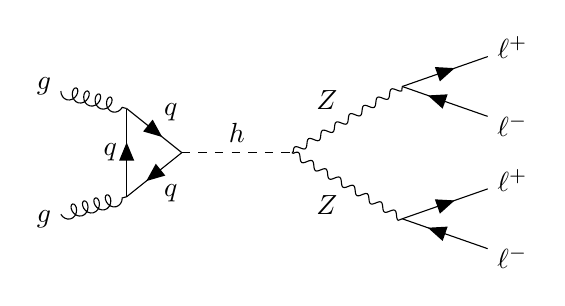
\begin{tikzpicture}[scale=0.7, every node/.style={transform shape=false}]
        \begin{feynman}
            % Gluon emission vertices
            \vertex (g1) at (-1.5,  1.2) {\(g\)};
            \vertex (g2) at (-1.5, -1.2) {\(g\)};
            
            % Triangle loop
            \vertex (loop1) at (0,  0.8);
            \vertex (loop2) at (0, -0.8);
            \vertex (loop3) at (1,  0.0);
            
            % Higgs
            \vertex (h)     at (3,  0.0);
            
            % Z bosons
            \vertex (z1)    at (5,  1.2);
            \vertex (z2)    at (5, -1.2);
            
            % Final leptons
            \vertex (l1)    at (7,  1.9) {\(\ell^+\)};
            \vertex (l2)    at (7,  0.5) {\(\ell^-\)};
            \vertex (l3)    at (7, -0.5) {\(\ell^+\)};
            \vertex (l4)    at (7, -1.9) {\(\ell^-\)};
            
            % Diagram
            \diagram*{
                (g1) -- [gluon] (loop1),
                (g2) -- [gluon] (loop2),
                
                (loop1) -- [fermion, edge label=\(q\)] (loop3),
                (loop3) -- [fermion, edge label=\(q\)] (loop2),
                (loop2) -- [fermion, edge label=\(q\)] (loop1),
                
                (loop3) -- [scalar, edge label=\(h\)] (h),
                
                (h) -- [boson, edge label=\(Z\)] (z1),
                (h) -- [boson, edge label'=\(Z\)] (z2),
                
                (z1) -- [fermion]      (l1),
                (z1) -- [anti fermion] (l2),
                (z2) -- [fermion]      (l3),
                (z2) -- [anti fermion] (l4),
            };
        \end{feynman}
    \end{tikzpicture}
    \caption{The Feynman diagram of Higgs boson decay in the four-lepton ``golden'' channel.}
    \label{fig:higgs}
\end{figure}

The Higgs boson can be produced in proton-proton collisions through the gluon fusion process, in which two gluons from the colliding protons interact via a top or bottom quark loop to generate a Higgs boson. These Higgs bosons, with the expected mass of $m_H \simeq 125\GeV$, can then decay into two $Z$ bosons, among other channels ($H \to WW$, $H \to bb$, and $H \to \tau \tau$)~\citep{Gunion1989}, one of which is considered off-shell, where the $Z$ boson is produced with a mass below its nominal mass of $91.2 \GeV$. Each $Z$ boson can then decay into a pair of lepton-antilepton, resulting in the final state of four leptons (electrons or muons). Figure \ref{fig:higgs} shows the Feynman diagram for this process. The decay of the Higgs boson into four leptons is regarded as the ``golden'' channel, as none of the final-state particles are neutrinos, which would result in missing energy and loss of information, or hadrons, which necessitate more complex modeling of jet fragmentation and hadronization. The invariant mass of the four-lepton system can be used to reconstruct the mass of the Higgs boson, allowing for a precise measurement of its properties.

\subsection{Background events}
\label{ssec:background_theory}

\begin{figure*}[htbp]
    \centering
    %------------------ First Row: (a), (b), (c) ------------------%
    \begin{minipage}{0.32\textwidth}
        \centering
        %%%%%%%%%%%%%%%%%%%%%%%%%%%%%%%%%%%%%%%%%%%%%%%%%%%%%%%%
        % (a) qq -> ZZ via s-channel gamma*/Z*
        %%%%%%%%%%%%%%%%%%%%%%%%%%%%%%%%%%%%%%%%%%%%%%%%%%%%%%%%
        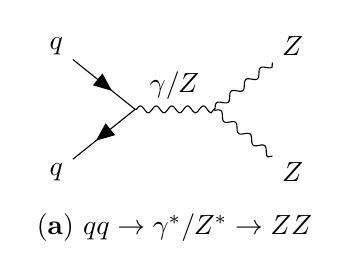
\begin{tikzpicture}
            \begin{feynman}
            % Define vertices
                \vertex (q1) at (-1,  0.8) {\(q\)};
                \vertex (q2) at (-1, -0.8) {\(q\)};
                \vertex (v)  at (0, 0);
                \vertex (w)  at (1, 0);
                \vertex (Z1) at (2,  0.8) {\(Z\)};
                \vertex (Z2) at (2, -0.8) {\(Z\)};
                
                % Diagram connections
                \diagram*{
                    (q1) -- [fermion] (v) -- [fermion] (q2),
                    (v) -- [boson, edge label = $\gamma / Z$] (w),
                    (w) -- [boson] (Z1),
                    (w) -- [boson] (Z2),
                };
            \end{feynman}
            % Label for diagram (a)
            \node at (0.5, -1.5) {(\textbf{a}) $qq \to \gamma^*/Z^* \to ZZ$};
        \end{tikzpicture}
    \end{minipage}
    \begin{minipage}{0.32\textwidth}
        \centering
        %%%%%%%%%%%%%%%%%%%%%%%%%%%%%%%%%%%%%%%%%%%%%%%%%%%%%%%%
        % (b) qq -> ZZ via t-channel quark exchange
        %%%%%%%%%%%%%%%%%%%%%%%%%%%%%%%%%%%%%%%%%%%%%%%%%%%%%%%%
        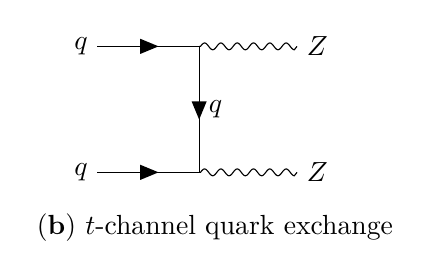
\begin{tikzpicture}
            \begin{feynman}
                % Define vertices
                \vertex (q1) at (-1.5, 0.8) {\(q\)};
                \vertex (q2) at (-1.5,-0.8) {\(q\)};
                \vertex (v1) at (0,  0.8);
                \vertex (v2) at (0, -0.8);
                \vertex (Z1) at ( 1.5,  0.8) {\(Z\)};
                \vertex (Z2) at ( 1.5, -0.8) {\(Z\)};
                
                % Diagram connections
                \diagram*{
                    (q1) -- [fermion] (v1) -- [boson] (Z1),
                    (q2) -- [fermion] (v2) -- [boson] (Z2),
                    (v1) -- [fermion, edge label=\(q\)] (v2),
                };
            \end{feynman}
            % Label for diagram (b)
            \node at (0.2, -1.5) {(\textbf{b}) $t$-channel quark exchange};
        \end{tikzpicture}
    \end{minipage}
    \begin{minipage}{0.32\textwidth}
        \centering
        %%%%%%%%%%%%%%%%%%%%%%%%%%%%%%%%%%%%%%%%%%%%%%%%%%%%%%%%
        % (c) qq -> ZZ via u-channel quark exchange
        %%%%%%%%%%%%%%%%%%%%%%%%%%%%%%%%%%%%%%%%%%%%%%%%%%%%%%%%
        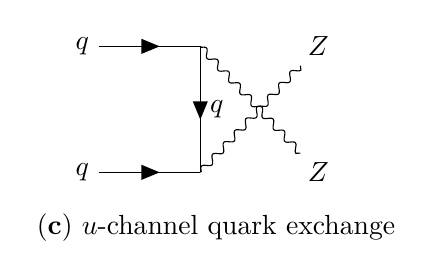
\begin{tikzpicture}
            \begin{feynman}
            % Define vertices
                \vertex (q1) at (-1.5, 0.8) {\(q\)};
                \vertex (q2) at (-1.5,-0.8) {\(q\)};
                \vertex (v1) at (0,  0.8);
                \vertex (v2) at (0, -0.8);
                \vertex (Z1) at ( 1.5,  0.8) {\(Z\)};
                \vertex (Z2) at ( 1.5, -0.8) {\(Z\)};
                
                % Connect so that final Z lines are "crossed"
                \diagram*{
                    (q1) -- [fermion] (v1) -- [boson] (Z2),
                    (q2) -- [fermion] (v2) -- [boson] (Z1),
                    (v1) -- [fermion, edge label=\(q\)] (v2),
                };
            \end{feynman}
            % Label for diagram (c)
            \node at (0.2, -1.5) {(\textbf{c}) $u$-channel quark exchange};
        \end{tikzpicture}
    \end{minipage}

    %------------------ Second Row: (d), (e) ------------------%
    \vspace{0.5cm}

    \begin{minipage}{0.32\textwidth}
        \centering
        %%%%%%%%%%%%%%%%%%%%%%%%%%%%%%%%%%%%%%%%%%%%%%%%%%%%%%%%
        % (d) gg -> ZZ box diagram #1
        %%%%%%%%%%%%%%%%%%%%%%%%%%%%%%%%%%%%%%%%%%%%%%%%%%%%%%%%
        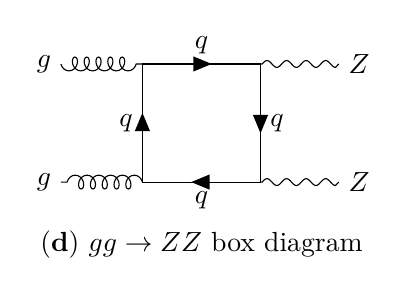
\begin{tikzpicture}
            \begin{feynman}
            % Vertices of the box
                \vertex (g1) at (-1.25, 1.5) {\(g\)};
                \vertex (v1) at ( 0, 1.5);
                \vertex (v2) at ( 1.5, 1.5);
                \vertex (g2) at (-1.25, 0) {\(g\)};
                
                \vertex (v3) at ( 0, 0);
                \vertex (v4) at ( 1.5, 0);
                
                % Z bosons on the right
                \vertex (Z1) at ( 2.75,  1.5) {\(Z\)};
                \vertex (Z2) at ( 2.75, 0) {\(Z\)};
                
                % Diagram
                \diagram*{
                    (g1) -- [gluon] (v1) -- [fermion, edge label=\(q\)] (v2),
                    (v2) -- [fermion, edge label=\(q\)] (v4),
                    (v4) -- [fermion, edge label=\(q\)] (v3)-- [gluon] (g2),
                    (v3) -- [fermion, edge label=\(q\)] (v1),
                    (v2) -- [boson] (Z1),
                    (v4) -- [boson] (Z2),
                };
            \end{feynman}
            % Label for diagram (d)
            \node at (0.75, -0.8) {(\textbf{d}) $gg \to ZZ$ box diagram};
        \end{tikzpicture}
    \end{minipage}
    \begin{minipage}{0.32\textwidth}
        \centering
        %%%%%%%%%%%%%%%%%%%%%%%%%%%%%%%%%%%%%%%%%%%%%%%%%%%%%%%%
        % (e) gg -> ZZ box diagram #2 (crossed)
        %%%%%%%%%%%%%%%%%%%%%%%%%%%%%%%%%%%%%%%%%%%%%%%%%%%%%%%%
        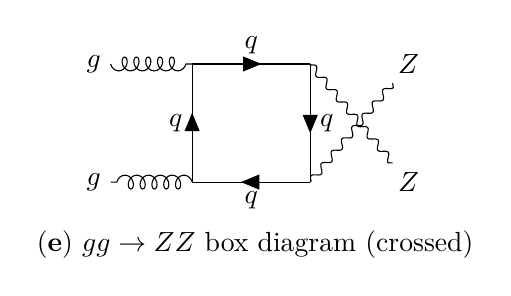
\begin{tikzpicture}
            \begin{feynman}
            % Vertices of the box
            \vertex (g1) at (-1.25, 1.5) {\(g\)};
            \vertex (v1) at ( 0, 1.5);
            \vertex (v2) at ( 1.5, 1.5);
            \vertex (g2) at (-1.25, 0) {\(g\)};
            
            \vertex (v3) at ( 0, 0);
            \vertex (v4) at ( 1.5, 0);
            
            % Z bosons on the right
            \vertex (Z1) at ( 2.75,  1.5) {\(Z\)};
            \vertex (Z2) at ( 2.75, 0) {\(Z\)};
            
            % Diagram
            \diagram*{
                (g1) -- [gluon] (v1) -- [fermion, edge label=\(q\)] (v2),
                (v2) -- [fermion, edge label=\(q\)] (v4),
                (v4) -- [fermion, edge label=\(q\)] (v3)-- [gluon] (g2),
                (v3) -- [fermion, edge label=\(q\)] (v1),
                (v2) -- [boson] (Z2),
                (v4) -- [boson] (Z1),
            };
            \end{feynman}
            % Label for diagram (e)
            \node at (0.8, -0.8) {(\textbf{e}) $gg \to ZZ$ box diagram (crossed)};
        \end{tikzpicture}
    \end{minipage}
    \caption{Feynman diagrams of the non-reducible $ZZ$ background processes via the $qq \to ZZ$ ({\bf a}--{\bf c}) and $gg \to ZZ$ ({\bf d}--{\bf e}) channels.}
    \label{fig:zz_background}
\end{figure*}

Despite the clear signature of the Higgs four-lepton channel, its branching fraction, i.e. the fraction of decays into a particular channel, is only about $2.8 \pm 0.3 \%$~\citep{PDG2024}. On top of the low production rate of the Higgs boson, this results in other background processes, producing similar final states, dominating observations. Most of these events, such as the production of a $Z$ boson through the Drell–Yan process~\citep{DrellYan1970} or lepton production of top–antitop interactions (in combination with jet misidentification, among other factors), are reducible through careful selection criteria for leptons, as discussed further in Section \ref{sec:experiment} and \ref{sec:background_suppression}. However, the most significant background processes, involving the same $ZZ$ decay channel as Higgs bosons, cannot be entirely eliminated. These processes, arising from interactions between quarks or gluons (as illustrated in Figure \ref{fig:zz_background}), necessitate further background suppression techniques, including analysis of Monte Carlo simulations and certain uses of neural networks.


\section{Experimental data}
\label{sec:experiment}

The CMS detector consists of a central solenoid magnet, which generates a magnetic field of 3.8 T, and a series of detectors designed to measure the charge, momentum, and energy of particles~\citep{CMS2008}. From the center outwards, the detector includes a silicon tracker, which measures the trajectories of charged particles, an electromagnetic calorimeter (ECAL), where the energies of photons and electrons are measured, and a hadronic calorimeter (HCAL), which measures the energies of hadrons. The outermost layer is a muon system, which identifies and measures the momentum of muons. The detector geometry is described in terms of the transverse angle $\phi$ and the pseudorapidity $\eta$, which is defined as $\eta = -\ln(\tan(\theta/2))$, where $\theta$ is the polar angle of the particle with respect to the beam axis. For measurements of charged particles, pseudorapidity is limited to $|\eta| < 2.5$, while for neutral particles, it is limited to $|\eta| < 3.0$. For muons, the pseudorapidity is limited to $|\eta| < 2.4$.

The data utilized in this analysis were collected during the 2011-2012 LHC run, with a center-of-mass energy of $\sqrt{s} = 7\TeV$ and $8\TeV$, respectively. In order to guide the analysis and event selection criteria, we also utilize Monte Carlo (MC) simulations of relevant events to model the signal and background processes (details on such simulations can be found in~\citep{CMS2012}). We select only events with four leptons (electrons or muons) in the final state through enforcing the transverse and longitudinal impact parameters with respect to the primary vertex to $| {\rm d}_{xy} | < 0.5\cm$ and $| {\rm d}_z | < 1.0\cm$, respectively. These impact parameters are defined as the closest distance between the particle trajectory and the primary vertex in the respective plane of reference. The three-dimensional impact parameter significances of the leptons, i.e. the impact parameter signal-noise ratios, are enforced to be less than 4.0, which ensures that the lepton pairs produced from $Z$ boson decays originate from the same primary vertex. We also require that the leptons are isolated from other particles in the events, which is achieved by requiring a maximum relative isolation of the lepton of 0.4 within the cone radius of $\Delta R = \sqrt{\left(\Delta \eta\right)^2 + \left(\Delta \phi\right)^2} = 0.4$. Here, relative isolation of the lepton is defined as the scalar sum of the transverse momenta of particles reconstructed within a distance $\Delta R$ of the lepton, divided by the transverse momentum of the lepton, with transverse momentum defined as $p_{\rm{T}} = \sqrt{p_x^2 + p_y^2}$, where $p_x$ and $p_y$ are the transverse components of the momentum vector. 


\section{Background suppression}
\label{sec:background_suppression}

Through the selection criteria detailed in Section \ref{sec:experiment}, we are able to select a sample of events with four leptons in the final state. However, as discussed in Section \ref{ssec:background_theory}, background processes that can mimic the signal remain as dominant sources of events. To suppress these background events, we utilize a combination of kinematic variables and machine learning techniques. The following selection criteria performance are evaluated within the context of MC simulations, serving as a guideline prior to the unblinding process.

First, we enforce charge conservation in the four-lepton system, which imposes the sum of charges in each event to be zero. This is a necessary condition for the production of a neutral Higgs boson. Additionally, leptons are required to have sufficient transverse momentum, specifically $p_{\rm{T}} \geq 7\GeV$ for electrons and $p_{\rm{T}} \geq 5\GeV$ for muons. As a result of these selection cuts, $90 \text{--} 95\%$ of the Drell-Yan and top-antitop background events (depending on the exact decay channels) are removed, while the signal efficiency remains above $90\%$. Taking into account the relative process luminosities, these background contributions from these processes are reduced to a negligible level. Nevertheless, the irreducible $ZZ$ background, of which only $20 \text{--} 30\%$ of events are removed through the cut, remains the dominant source of background. As the remaining four-lepton events are mainly produced through the same $ZZ$ decay channel, we pair up the particles into lepton-antilepton pairs and reconstruct the invariant masses of the Z bosons. The invariant mass is calculated as $m = \sqrt{\left(\sum_i E_i\right)^2 - \left(\sum_i \vec{p}_i\right)^2}$, where $E_i$ and $\vec{p}_i$ are the energy and momentum vector of the particle, respectively. Following~\citep{CMS2012}, we require that the mass of the heavier Z boson be within the range of $40 \text{--} 120\GeV$, while the mass of the lighter Z boson is required to be within $12 \text{--} 120\GeV$. This removes an additional $25\%$ of the background events, while maintaining a signal efficiency of $95\%$.

In order to further remove background events, we utilize a fully-connected Graph Convolutional Network (GCN)~\citep{KipfWelling2016} with each lepton as a node in the graph. The network is trained to perform event classification, distinguishing between signal and background. Each node is characterized by the particle type, encoded through a trainable embedding layer, and transverse momentum, which together serve as the input features for the model. The GCN architecture is designed to preserve symmetry between leptons while avoiding bias towards specific four-lepton invariant masses. Nevertheless, to avoid the $91.2 \GeV$ Z boson peak, the network is trained exclusively on data within the invariant mass range of $100 \text{--} 160\GeV$. We argue that this does not cause further bias in the selection, compared to the already-biased single choice of Higgs mass in the simulations. The optimal GCN model is selected based on the detection and false alarm rates, as well as the concentration of background removal. Using the model, we are able to remove an additional $70\%$ of the background events, while maintaining a signal efficiency of $80\%$. The resulting prominence of the signal peak compared to the surrounding background count is around 5, which should be sufficient to observe the Higgs boson, given that the theory is correct.


\section{Data analysis \& Results}
\label{sec:result}

\begin{figure}
    \centering
    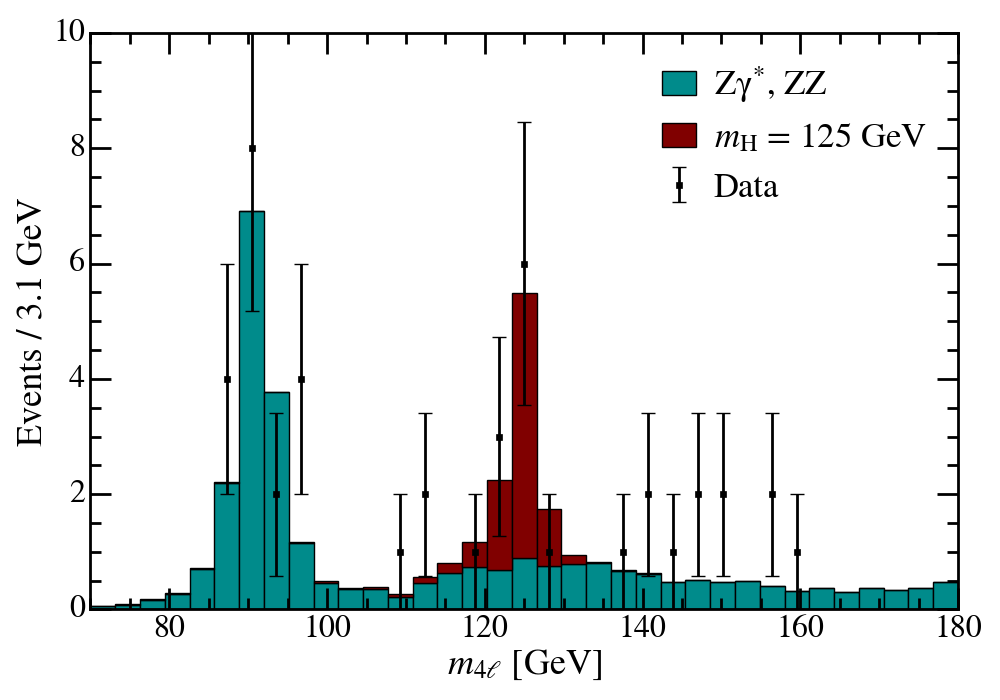
\includegraphics[width=0.49 \textwidth]{Figures/event_histogram.png}
    \caption{Distribution of the four-lepton invariant mass $m_{4\ell}$ in the selected events. The red and cyan solid histograms represent the expected contributions from the Higgs boson signal with $m_H = 125,\GeV$ and the irreducible $ZZ$ background, respectively. The observed event counts from the CMS 2011–2012 dataset are shown as black error bars.}
    \label{fig:event_histogram}
\end{figure}

\begin{figure}
    \centering
    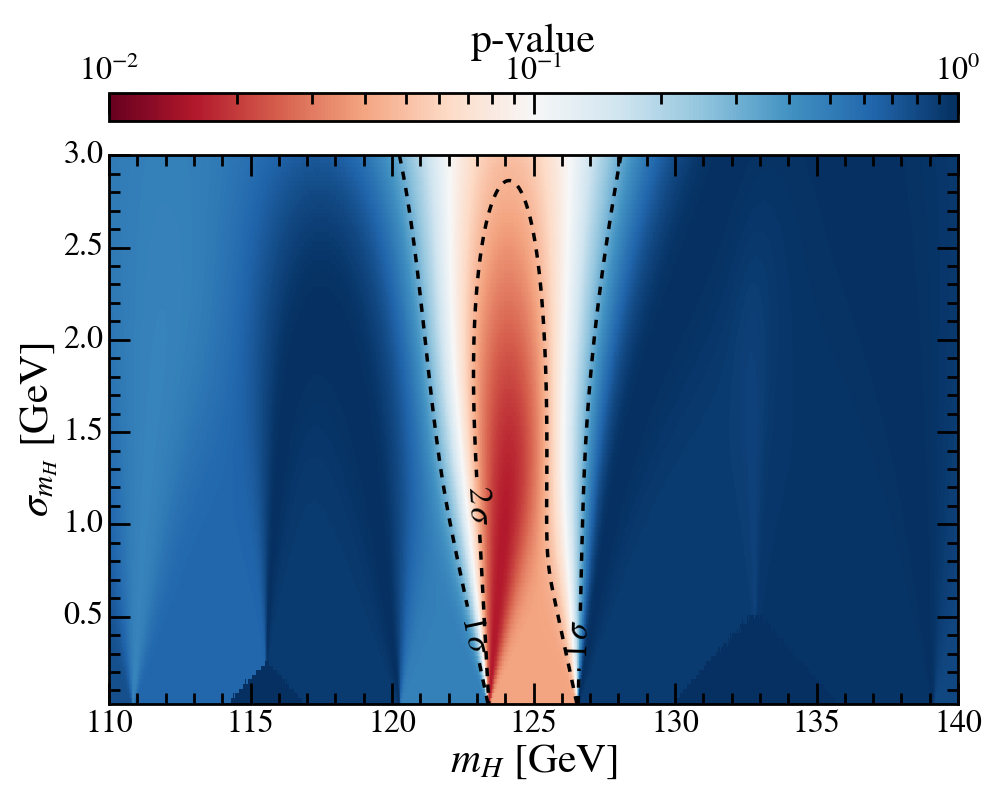
\includegraphics[width=0.49 \textwidth]{Figures/p-value.png}
    \caption{The p-value as a function of the Higgs boson mass $m_H$ and four-lepton signal characterized standard deviation width $\sigma_{m_H}$. The dashed contours indicate the regions corresponding to $1\sigma$ and $2\sigma$ significance levels. Although $\sigma_{m_H}$ is held fixed during each individual regression, the p-value is evaluated under the assumption that $\sigma_{m_H}$ is a free parameter in the overall hypothesis test.}
    \label{fig:p-value}
\end{figure}

Figure \ref{fig:event_histogram} presents the distribution of the four-lepton invariant mass $m_{4\ell}$ for the selected events. The observed data from CMS appear to be consistent with the expected counts derived from the Monte Carlo (MC) simulated events. A bin width of $3.1,\GeV$ is adopted for the histogram to balance resolution with statistical reliability, ensuring a reasonable number of events per bin. However, due to the overall low event counts, statistical uncertainties remain significant. To further investigate the potential Higgs boson signal, we conduct a hypothesis test. The null hypothesis corresponds to the absence of a Higgs boson signal, while the alternative hypothesis includes a Higgs signal component. Under the null hypothesis, the distribution of $m_{4\ell}$ is modeled using the background expectation from the MC simulations, scaled by a constant normalization factor. For the alternative hypothesis, the background model remains unchanged, and the signal is approximated by a Gaussian peak, centered at a variable Higgs mass $m_H$ and characterized by a standard deviation $\sigma_{m_H}$.

The p-value, representing the probability of observing a signal assuming the null hypothesis is true, is evaluated as a function of $m_H$. This involves fitting both signal and background models to the observed data. Due to the low event counts, we adopt a Poisson likelihood approach for the fitting procedure. To simplify the analysis, we perform a grid search over fixed values of $\sigma_{m_H}$ within the range $0.1 \text{--} 3.1,\GeV$, as suggested by the observed distribution. The resulting p-values, shown in Figure \ref{fig:p-value}, are computed from the difference in log-likelihoods between the null and alternative hypotheses. While $\sigma_{m_H}$ is fixed during each fit, the p-values are interpreted under the assumption that it is a free parameter.

A clear minimum in the p-value distribution is observed at $m_H \simeq 123.8,\GeV$, with a corresponding p-value of $0.016$, indicating a local significance of approximately $2.4\sigma$. A change in the standard deviation $\sigma_{m_H}$ does not significantly affect the p-value, as the distribution remains relatively flat. This suggests that the observed signal is robust against variations in the width of the Gaussian peak. To obtain a more precise estimate of the Higgs mass and its associated uncertainty, we employ a bootstrapping procedure. The observed data are resampled by perturbing the event counts according to their respective uncertainties, followed by a repetition of the analysis on each resampled dataset. This yields an estimated Higgs mass of $m_H = 124.22 \pm 1.16,\GeV$, which is in good agreement with the expected value of $m_H \simeq 125,\GeV$.


\section{Discussion \& Conclusion}
\label{sec:discussion}

In this study, we report an observation of the Higgs boson via the four-lepton decay channel, using data collected during the 2011–2012 run of the CMS experiment at the LHC. The analysis employs a combination of kinematic selection criteria and machine learning techniques to effectively suppress background contributions, leading to the emergence of a statistically significant signal peak in the four-lepton invariant mass distribution. A significance of $2.4\sigma$ is achieved, and the Higgs boson mass is measured to be $m_H = 124.22 \pm 1.16,\GeV$. This measurement is consistent with prior results and constitutes additional evidence supporting the existence of the Higgs boson.

Despite the encouraging results, several limitations remain. First, the analysis is restricted to a single decay channel, which, while clean and well-reconstructed, may not capture the full phenomenological breadth of Higgs boson production and decay. Second, the modeling of background processes using Monte Carlo (MC) simulations shows some discrepancies with the observed data, as illustrated in Figure \ref{fig:event_histogram}, suggesting potential shortcomings in the simulation or in the treatment of systematic uncertainties. Additionally, the focus on testing a single mass hypothesis may introduce bias, particularly in the presence of low statistics and imperfect background modeling. Future work should aim to refine the modeling of both signal and background processes, as well as expand the analysis to include additional Higgs decay channels and production modes. Furthermore, the application of more advanced machine learning methods may enhance the sensitivity of future searches by further improving background rejection and optimizing signal extraction.


\begin{acknowledgments}

The author thanks his lab partner Y. Hu for collaboration in the experiment. Special thanks to the JLab teaching staff, P. Lugato, for their guidance and support, as well as CERN Open Data for providing the experimental data.

\end{acknowledgments}

%%%%%%%%%%%%%%%%%%%%%%%%%%%%%%%%%%%%%%%%%%%%%%%%%%%%%%%%%%%%%%%%%%

\bibliography{ref}

%%%%%%%%%%%%%%%%%%%%%%%%%%%%%%%%%%%%%%%%%%%%%%%%%%%%%%%%%%%%%%%%%%

\end{document}